\style{mb} %pour microbit


\section{Fluctuation d'échantillonnage avec \mb}


\subsection{Description}

\subsubsection{Objectif}


%   bloc de formule
%   sans titre et fond bleu cyan
\begin{formule}
Le but de ce projet est d'expérimenter la fluctuation d'échantillonnage à  partir d'une situation classique, en établissant tout d'abord un modèle d'expérience aléatoire à partir des données de la situation, puis en proposant de programmer le tirage d'échantillons pour une taille n fixée.
\end{formule}


\subsubsection{Intérêt}

 L'utilisation de l'interface \mb permet d'obtenir rapidement un programme fonctionnel, mais aussi d'afficher graphiquement la série de données produites par le simulateur. Cela représente un intérêt non-négligeable lorsque l'on souhaite traiter la fluctuation d'échantillonnage.

%liste d'arguments
\begin{description}
    \item [Simulation d'une grande série d'expériences aléatoires] Contrairement à l'usage du tableur, où l'élève va devoir manipuler un grand nombre de données en colonnes et en lignes, au risque de se perdre dans leur traitement, l'approche algorithmique de  ce problème permet d'aller à l'essentiel.
    \item [Afficher les données]
    L'utilisation de l'interface \mb permet d'obtenir rapidement un programme fonctionnel, mais aussi d'afficher graphiquement la série de données produites par le simulateur. Cela représente un intérêt non-négligeable lorsque l'on souhaite traiter la fluctuation d'échantillonnage.
\end{description}


\subsubsection{Matériel}
\begin{itemize}
%   matériel pour micro:bit
    \item 1 $\times$ \matosMb \emph{(facultatif car le simulateur peut suffire)}
%   site pour micro:bit
    \item 1 $\times$ accès internet : IDE programmation par bloc \url{http://makecode.microbit.org/}
    \item lien vers l'activité 1 : \url{https://makecode.microbit.org/_TbPFTK8eaKes}
    \item lien vers l'activité 2 : \url{https://makecode.microbit.org/_PW8LCg82z3fh}
    \item lien vers l'activité 3 :
    \url{https://makecode.microbit.org/_11aUTkWzR60J}
\end{itemize}

\newpage

\subsubsection{Progression proposée}


%   bloc méthode
%   titre + fond bleu
\begin{methode}
    On propose ici d'aborder la problématique en trois temps :
    
    \begin{enumerate}
        \item \textbf{Prise en main - Vérifier le modèle.} \\
            Pour faciliter la prise en main et gagner du temps on propose aux élèves de vérifier un code déjà prêt. Cela facilite l'appropriation du problème.
        \item \textbf{Intermédiaire - Du modèle à la génération d'échantillons.}\\
            À partir du modèle, l'élève doit élaborer un algorithme afin de produire des échantillons de taille fixé.
        \item \textbf{Avancé - Visualisation des données}\\
            Cette étape consiste en une amélioration du programme précédent afin de pouvoir visualiser les données issues de la simulation.
            
    \end{enumerate}
\end{methode}

%
% activité de niveau 1
%

%   saut de page
\newpage

%   titre de la sous section
\subsection{Niveau prise en main - Vérifier le modèle\ldots}

\subsubsection{Activité élève}

% commande perso \CARTOUCHE
%   5 paramètres : 
%       * durée
%       * public
%       * travail en maths
%       * travail en sciences
%       * travail en algo
\cartouche
{0,3 h}         %durée
{première}           %public
{statistiques et probabilités}        %maths
{}     %sciences
{instruction conditionnelle}       %algo


%   petite image de logo qui va
%   se mettre dans le bloc élève
\begin{wrapfigure}{r}{3cm}
    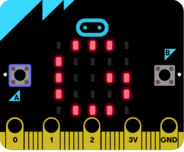
\includegraphics[width=\linewidth]{res/mb-fluctuations-illustration.png}
\end{wrapfigure}

%   bloc élève
%   fond orange
\begin{eleve}    
    \texttt{\textsc{Ta Mission} : Utiliser \mb pour simuler des \emph{naissances}!}
    
    La situation est la suivante : à Ufa, en Russie, 51,2 \%  des naissances sont des garçons.
    
    Dans cette ville, une usine agrochimique expose ses employés à des pesticides contenant de la dioxine.
    
    D’après une étude de l’université de Montréal, parmi les 227 enfants nés d’un parent travaillant dans cette usine, 91 sont des garçons.
    
    Cette étude cherche à déterminer si l’usine interfère sur les naissances.
    
    Pour simuler les naissances à Ufa, on propose d'utiliser le programme ci-dessous.
    
    \emph{Expliquer pourquoi} ce programme modélise correctement les naissance à Ufa.
    
    \emph{Proposer} une façon de l'exploiter afin de vérifier l'influence des produits chimiques sur les naissances.
    
%   ajout d'une image
    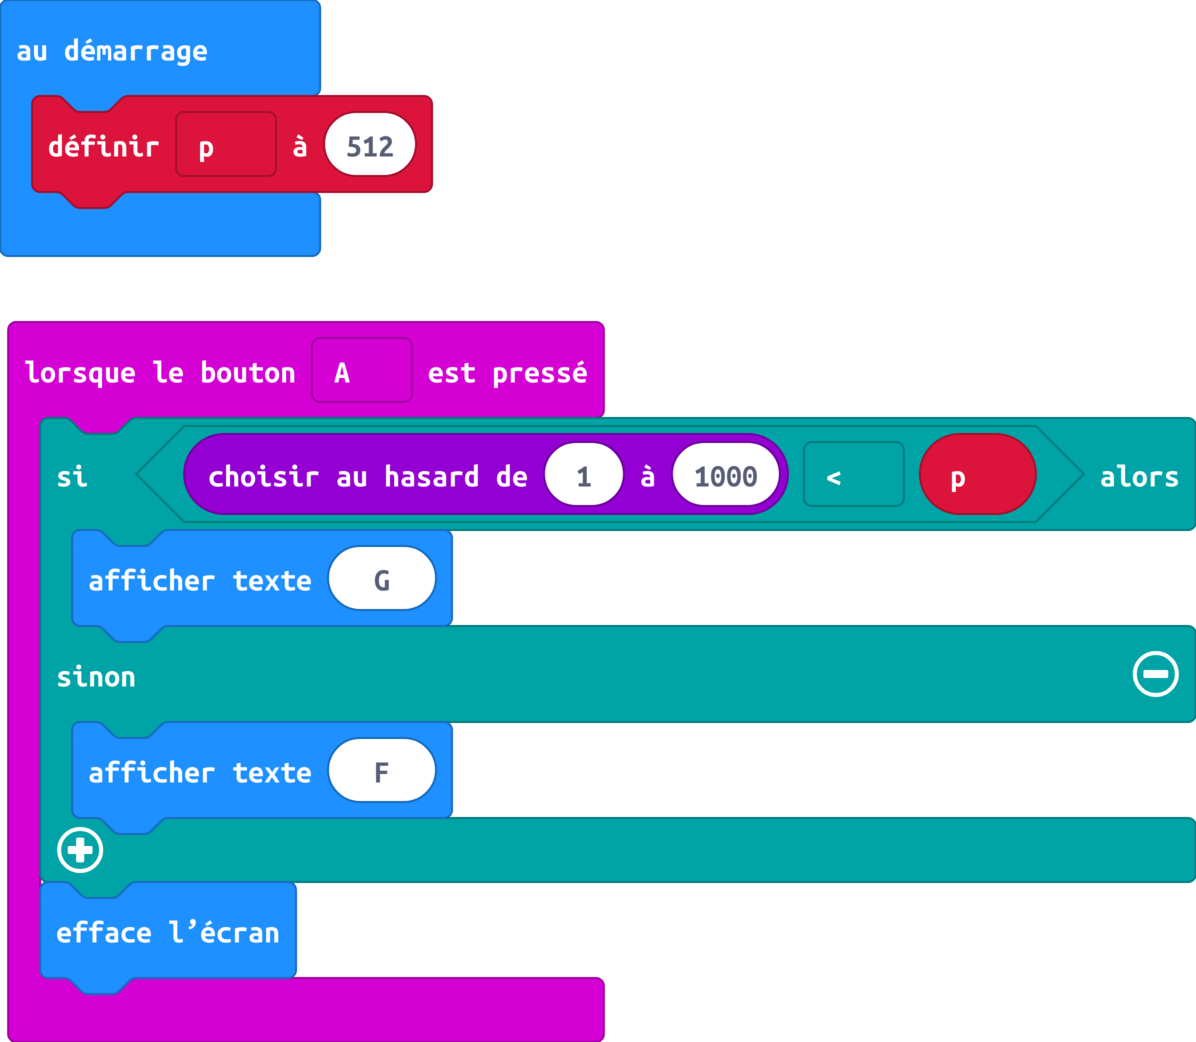
\includegraphics[width=0.5\linewidth]{res/mb-fluctuation-activite1.png}
    
\end{eleve}



\subsubsection{Notes pour l'enseignant}

%
%   méthode et remarque
%
\begin{methode}
Dans cette activité, il s'agit de vérifier que les élèves ont bien compris la problématique et notamment comment est utilisé la fréquence d'apparition du caractère "garçon".

Bien entendu il faut suggérer aux élèves de tester le programme, afin d'en appréhender les limites.
\end{methode}


\begin{remarque}
    Ici l'utilisation de la variable \emph{p} n'est pas indispensable pour l'algorithme. Son intérêt est pédagogique : elle permet de mettre en évidence la donnée utilisée ainsi que de de faire le lien avec le vocabulaire et les notations utilisées dans le cours.

   Avant de passer à l'activité 2, il peut être préférable de lister avec les élèves les éléments manquants qui permettraient de produire et de traiter un échantillon comparable à celui de l'étude :
   \begin{itemize}
       \item une boucle répéter afin de produire un échantillon de taille 227
       \item des variables pour dénombrer les naissances de garçons (et de filles ?)
   \end{itemize}
\end{remarque}

%
% activité de niveau 2
%

%   saut de page
\newpage

%   titre de la sous section
\subsection{Niveau intermédiaire - Générer des échantillons\ldots}

\subsubsection{Activité élève}

% commande perso \CARTOUCHE
%   5 paramètres : 
%       * durée
%       * public
%       * travail en maths
%       * travail en sciences
%       * travail en algo
\cartouche
{0,5 h}         %durée
{première}           %public
{statistiques et probabilités}        %maths
{}     %sciences
{instruction conditionnelle; boucle}       %algo


%   petite image de logo qui va
%   se mettre dans le bloc élève
\begin{wrapfigure}{r}{3cm}
    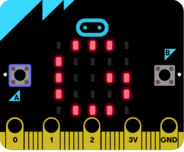
\includegraphics[width=\linewidth]{res/mb-fluctuations-illustration.png}
\end{wrapfigure}

%   bloc élève
%   fond orange
\begin{eleve}    
    \texttt{\textsc{Ta Mission} : Utiliser \mb pour simuler des \emph{naissances}!}
    
    Utilise les blocs proposés afin de générer des échantillons de taille identique à celui de l'étude.
    
    \emph{Construire} un programme qui affiche le nombre de garçons obtenus dans un échantillons de 227 naissances.
    
    \emph{Utiliser} le programme afin de vérifier si la situation de la problématique est vraisemblable.
    
%   ajout d'une image
    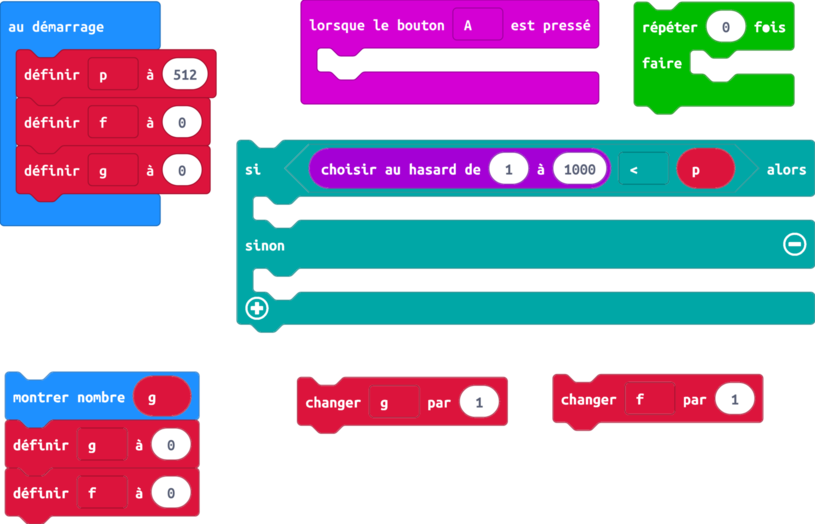
\includegraphics[width=0.8\linewidth]{res/mb-fluctuation-activite2-blocs.png}
    
\end{eleve}

%   saut de page
\newpage

\subsubsection{Notes pour l'enseignant}

%
%   méthode et remarque
%
\begin{methode}
Dans cette activité, il s'agit de vérifier que les élèves se sont bien appropriés la problématique, notamment par rapport à la taille de l'échantillon.

Bien entendu il faut suggérer aux élèves de tester le programme plusieurs fois.

Le programme attendu peut être celui-ci si l'élève a utilisé tous les blocs proposés (voir \emph{Remarque} ci-dessous) :

%   ajout d'une image
    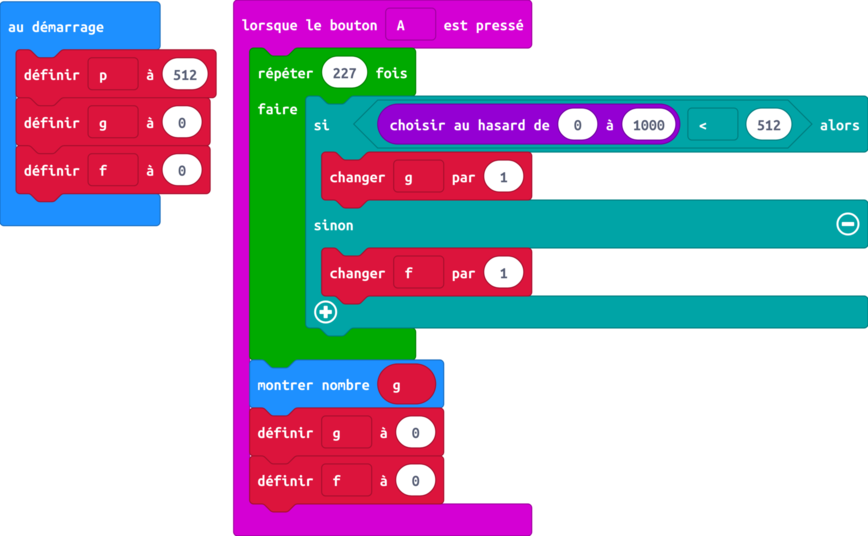
\includegraphics[width=0.8\linewidth]{res/mb-fluctuation-activite2-proposition.png}

\end{methode}


\begin{remarque}
    Ici l'utilisation de la variable \emph{f} n'est pas indispensable pour l'algorithme. Son intérêt est pédagogique : elle permet de faire le lien avec l'activité précédente en conservant le modèle proposé.

   Avant de passer à l'activité 3, il est tout de même préférable de faire s'interroger les élèves sur la nécessité de l'existence de la variable \emph{f}.
   
   Enfin, on interrogera les élèves sur le nombre d'échantillons qu'ils jugent nécessaires afin de valider leurs hypothèses.
\end{remarque}


%
% activité de niveau 3
%

%   saut de page
\newpage

%   titre de la sous section
\subsection{Niveau avancée - Produire des données\ldots}

\subsubsection{Activité élève}

% commande perso \CARTOUCHE
%   5 paramètres : 
%       * durée
%       * public
%       * travail en maths
%       * travail en sciences
%       * travail en algo
\cartouche
{0,5 h}         %durée
{première}           %public
{statistiques et probabilités}        %maths
{}     %sciences
{boucles imbriquées; communication}       %algo


%   petite image de logo qui va
%   se mettre dans le bloc élève
\begin{wrapfigure}{r}{3cm}
    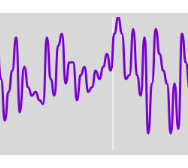
\includegraphics[width=\linewidth]{res/mb-fluctuation-activite3-illus.png}
\end{wrapfigure}

%   bloc élève
%   fond orange
\begin{eleve}    
    \texttt{\textsc{Ta Mission} : Utiliser \mb pour simuler des \emph{naissances} et produire des \emph{données}!}
    
    Utilise les blocs proposés afin de générer 100 échantillons de taille identique à celui de l'étude.
    
    \emph{Construire} un programme qui envoie une série de 100 valeurs, chacune correspondant au nombre de garçon dans un échantillon.
    
    \emph{Utiliser} le programme et la fonctionnalité \emph{Afficher la console} du simulateur pour visualiser les données.
    
    \emph{Exploiter} les données produites pour déterminer si l'usine interfère sur les naissances de garçons.
    
%   ajout d'une image
    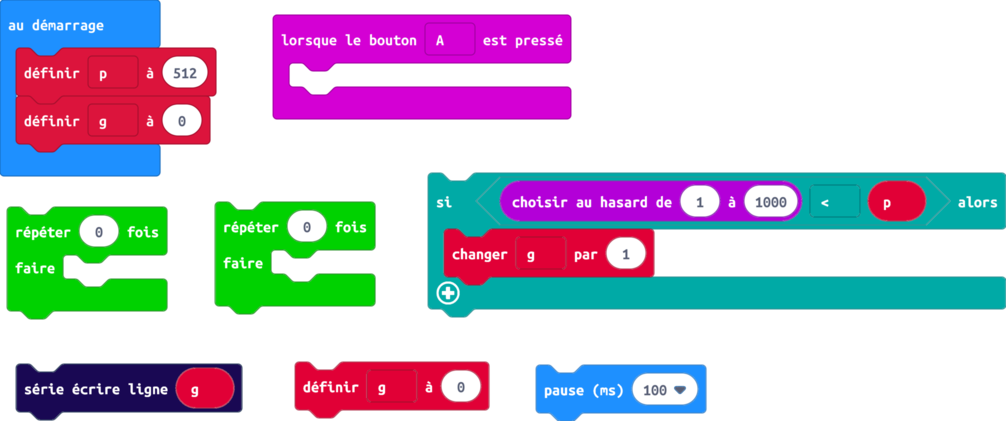
\includegraphics[width=0.8\linewidth]{res/mb-fluctuation-activite3-blocs.png}
    
\end{eleve}

%   saut de page
\newpage

\subsubsection{Notes pour l'enseignant}

%
%   méthode et remarque
%
\begin{methode}
Dans cette activité, il s'agit de vérifier que les élèves sont bien capable d'interpréter le graphique obtenu.

Bien entendu il faut suggérer aux élèves de tester le programme plusieurs fois, en prenant soin d'attendre la fin d'une série avant d'en lancer une deuxième

Le programme attendu peut être celui-ci  :

%   ajout d'une image
    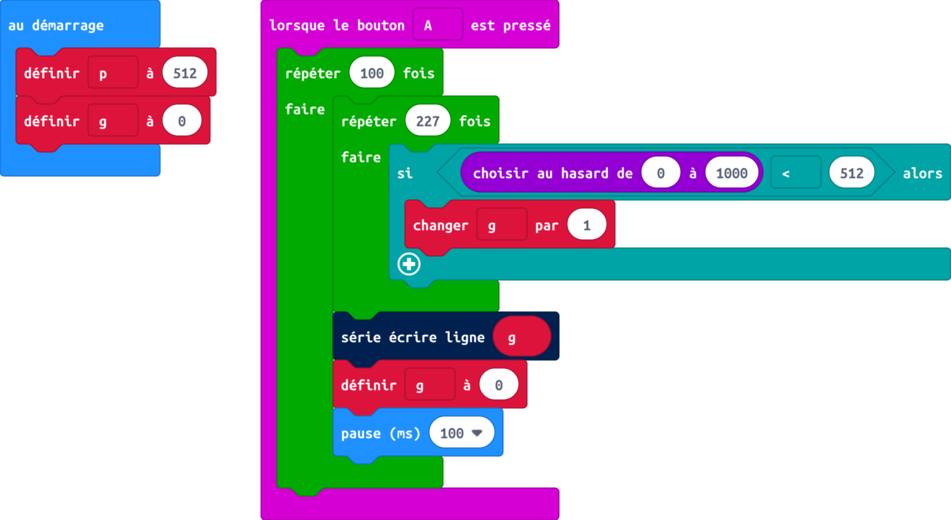
\includegraphics[width=0.8\linewidth]{res/mb-fluctuation-activite3-proposition.png}

\end{methode}


\begin{remarque}
   On interrogera les élèves sur les minimum et les maximum observés et sur la fréquence d'apparition d'un effectif inférieur ou égal à 91.
   
   Les données produites sont exportables en .csv et donc exploitables dans un tableur.
\end{remarque}
